\section{REST API: Week Schedule}\label{sec:restws}
This section pertains to the following user story: \\
\userstory{As a developer I would like an endpoint for Week Schedules, such that I can retrieve them from GIRAF.} \\
Specifically the two sub tasks regarding the core layer and the persistence layer, as they are done first, and we wont have time in this sprint to develop the service layer.

For the sake of this section, we refer to both the classes and also the real life objects that they represent, as such we make a distinction between how the two are written.
For when a class is referred to we write it as the class name and in a monospaced font, e.g. \texttt{WeekSchedule}.
If we refer to the object that it identifies in the real world it will be written in standard language grammar with our normal font, e.g. week schedule.\todo{Skal det ikke rykkes til noget forord/reading guide?}

\noindent
One of the focus points for this years GIRAF project have been the Week Schedule app.
The data for this application should be shared across devices, and some information across users.
Therefore it is crucial that the Week Schedule part of GIRAF is also part of its REST API.
This Section will explain the layers of the REST API for Week Schedule we developed during this sprint; the Core and Persistence layers. 

\subsection{Core}
In this subsection we will introduce the model we made in the core layer of the REST API.
First we will explain what this is meant to be used for and how it is currently modelled in the Week Schedule app, finally we will explain our solution to the problem. 

In the Week Schedule app the view is split into seven views, each representing a day of the week.
In the current version this is modelled as the Week Schedule being a sequence containing seven sequences.
Each of these views contain an ordered list of a combination of pictograms, sequences and choices.
As explained earlier we model these as the \texttt{Frame}--superclass, from which they all inherit. % They inherit despite noone dying. 
Each frame in a week schedule additionally have a number of boolean values that determine their progress, which indicates the status of the frame. 
The booleans that currently exist denote the progress are: Complete, Active, NotComplete and Cancelled. 
As mentioned this progress is not stored on the server, but on a locally saved file.
Since the progress information is personal, each user needs to separately have this information stored. 
As we believed some of the design choices to be odd, for our own design choices, we decided to base it upon how the Week Schedule app is used, and disregard the current model.

\begin{figure}
    \centering
        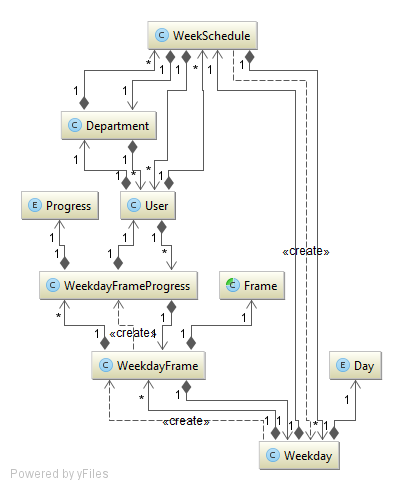
\includegraphics[width=0.8\textwidth]{figures/weekscheduleclassdiagram.png}
    \caption{The Class Diagram without their fields of classes involved with \texttt{WeekSchedule}.}\label{fig:weekscheduleclassdiagram}
\end{figure}

\myref{fig:weekscheduleclassdiagram} shows the class diagram of the classes involved with \texttt{WeekSchedule}.
A \texttt{WeekSchdule} has many \texttt{Weekday}s, although we allow no more than 7, and these are assigned an enum \texttt{Day} which indicates which day of the week the \texttt{Weekday} belongs to.
A \texttt{Weekday} have a number of \texttt{Frame}s as seen by the join-table \texttt{WeekdayFrame}.
These \texttt{WeekdayFrame}s are then involved with a \texttt{User} and each \texttt{User} has their own \texttt{Progress} which is all joined in the join-table \texttt{WeekdayFrameProgress}.
And then of course a \texttt{User} is able to have many \texttt{WeekSchedule}s which is also the case for a \texttt{Department}.
The following sections will introduce the fields of the classes created for modelling \texttt{WeekSchedule}.

\todo[inline]{Måske vi skal snakke om primary keys her med henblik på database senere eller skal vi det der? - Troels --- Er ikke med på hvad du mener? Nævne at Id er primary key ? - Søren}
\subsubsection{Week Schedule}
\myref{tbl:WeekSchedule} provides an overview of how we model a \texttt{WeekSchedule} in the REST API.
For some of the fields further details and thoughts behind their creation is provided.
The \texttt{WeekSchedule} class is central to the modelling of week schedules.
All information about a week schedule can be derived from this class, we will start by presenting this class and then following its fields to find the objects of types \texttt{Weekday}, \texttt{WeekdayFrame} and lastly \texttt{WeekdayFrameProgress}.

\begin{table}[ht]
\resizebox{\textwidth}{!}{%
    \centering
    \begin{tabular}{lll}
        \multicolumn{3}{c}{\Large{Class: \texttt{WeekSchedule}}}                                                                                \\
        \tblgrpsep
        \tblgrpsep
        \textbf{Field Name} & \textbf{Type}                                     & \textbf{Short Description}                                    \\
        \midrule
        \texttt{id}         & \texttt{long}                                     & Unique Identifier                                             \\
        \texttt{name}       & \texttt{string}                                   & Name of the \texttt{WeekSchedule}                             \\
        \texttt{thumbnail}  & \texttt{Pictogram}                                & The pictogram shown as thumbnail                              \\
        \texttt{lastEdit}   & \texttt{Date}                                     & Timestamp for when the \texttt{WeekSchedule} was last edited  \\
        \texttt{department} & \texttt{Department}                               & The department that owns the \texttt{WeekSchedule}            \\
        \texttt{users}      & \texttt{Collection\textless User\textgreater}     & All users for whom the \texttt{WeekSchedule} is available     \\
        \texttt{days}       & \texttt{Collection\textless Weekday\textgreater}  & The \texttt{weekday}s belonging to the \texttt{WeekSchedule}           
    \end{tabular}}
    \caption{Table of fields in the \texttt{WeekSchedule} class.}
    \label{tbl:WeekSchedule}
\end{table}
\todo[inline]{Har gjort dem viewable nu, er ikke sikker på om overskriften skal være deri, det er jo captionens job? - Troels}

\noindent
The fields id, name and thumbnail are fairly straight forward and thus will not be discussed further.
These kind of self--explanatory fields exist for all the following classes, in general we will not go into detail with id, name and similar simple fields as their names combined with the short description is sufficient for them to be understood, so if a field is omitted from further description it is because we deem it self explanatory.
\begin{description}
    \item [\texttt{lastEdit}] \hfill \\ 
    The \texttt{lastEdit} field serves the same purpose as \texttt{lastEdit} previously described in \myref{sec:pictogramendpoint}.
    \item [\texttt{department}] \hfill \\
    The \texttt{department} field is used to restrict access such that only users that are part of the \texttt{department} that owns the \texttt{WeekSchedule}, can access that \texttt{WeekSchedule}.
    \item [\texttt{users}] \hfill \\
    The \texttt{users} field defines which users the \texttt{WeekSchedule} is used by.
    The users in this collection pertains specifically to citizens as all guardians within a department can edit week schedules belonging to that department.
    This field allows for several citizens to use the same week schedule such that if the department goes on a trip, rather than having to create a week schedule for each individual citizen, they can use a shared one for shared activities.
    This is a feature not available in the live version of the system, yet it is something that the customers expressed a want for in our first meeting with them, the notes from said meeting is available at \citep{GIRAF20161stMeeting}.
    \item [\texttt{days}] \hfill \\
    The \texttt{days} field contains at most seven days which are represented by their own class, Weekday, described next.
    If a day is without activity it may be represented as either a Weekday, or lack thereof as an empty day does not require any information to create the view in the app.
\end{description}

\subsubsection{Weekday}
A \texttt{WeekSchedule} that has had any pictograms added to any related \texttt{Weekday}s, contains between one and seven \texttt{Weekdays}.
These \texttt{Weekdays} instances represent a single day of the week and contain information about the activities on a given day.
\myref{tbl:Weekday} provides an overview of how we model a weekday in the REST API.

\begin{table}[ht]
\resizebox{\textwidth}{!}{%
    \centering
    \begin{tabular}{lll}
        \multicolumn{3}{c}{\Large{Class: \texttt{Weekday}}}                                                                                \\
        \tblgrpsep
        \tblgrpsep
        \textbf{Field Name} & \textbf{Type}                                     & \textbf{Short Description}                                    \\
        \midrule
        \texttt{id}           & \texttt{long}                                   & Unique Identifier                                             \\
        \texttt{day}          & \texttt{Enum\textless Day\textgreater}          & Defines which day of the week the \texttt{Weekday} represents \\
        \texttt{lastEdit}     & \texttt{Date}                                   & Timestamp for when the \texttt{Weekday} was last edited       \\
        \texttt{weekSchedule} & \texttt{WeekSchedule}                           & The \texttt{WeekSchedule} the \texttt{Weekday} belongs to     \\
        \texttt{frames}       & \texttt{List\textless WeekdayFrame\textgreater} & An ordered list of WeekdayFrames 
    \end{tabular}}
    \caption{Table of fields in the \texttt{Weekday} class.}
    \label{tbl:Weekday}
\end{table}

\begin{description}
    \item [\texttt{lastEdit}] \hfill \\
    Having a \texttt{lastEdit} field on each \texttt{Weekday} as well as on each \texttt{WeekSchedule} allows for more specific information. 
    As such conflicts, as defined in \myref{ssec:policy}, are less likely to occur as the changes have to be targeted on the same Weekdays and not simply the \texttt{WeekSchedule}. 
    The lastEdit on \texttt{WeekSchedule} remains such that if no conflict occurs we will not have to check the \texttt{lastEdit} for each \texttt{Weekday} on a \texttt{WeekSchedule}.
    \item [\texttt{weekSchedule}] \hfill \\
    The \texttt{weekSchedule} field defines the \texttt{WeekSchedule} that a \texttt{Weekday} belongs to, a \texttt{Weekday} can only belong to a single \texttt{WeekSchedule}.
    Allowing for \texttt{Weekday}s to be shared among \texttt{WeekSchedule}s would create more opportunities for the aforementioned conflicts to occur and in a more complicated manner, as such we choose not to allow this.
    \item [\texttt{frames}] \hfill \\
    The \texttt{frames} field is a list used to contain \texttt{Frame}s on a \texttt{Weekday}.
    For this we use a class made specifically for linking \texttt{Frame}s and \texttt{Weekday}s together, \texttt{WeekdayFrame}.
    We use a list for this such that we can order the elements.
\end{description}

\subsubsection{WeekdayFrame}
In order to model that a pictogram has been added to day in the week schedule we use the \texttt{WeekdayFrame} class.
This class serves as the link between a \texttt{Weekday} and a \texttt{Frame}.
It is necessary that we have this intermediary class such that we can add additional information, in this case this information is ordering the \texttt{Frame}s in a list while allowing them to be reordered easily.
We also need the class such that we can create a relation from this class to the class \texttt{WeekdayFrameProgress}.
\myref{tbl:WeekdayFrame} provides an overview of how we model a weekday in the REST API.

\begin{table}[ht]
\resizebox{\textwidth}{!}{%
    \centering
    \begin{tabular}{lll}
        \multicolumn{3}{c}{\Large{Class: \texttt{WeekdayFrame}}}                                                                      \\
        \tblgrpsep
        \tblgrpsep
        \textbf{Field Name}         & \textbf{Type}         & \textbf{Short Description}                                              \\
        \midrule
        \texttt{id}                 & \texttt{long}         & Unique Identifier                                                       \\
        \texttt{weekday}            & \texttt{Weekday}      & The \texttt{Weekday} that a \texttt{Frame} should be added to           \\
        \texttt{frame}              & \texttt{Frame}        & The \texttt{Frame} that should be added to the \texttt{Weekday}         \\
        \texttt{index}              & \texttt{int}          & The order for which \texttt{Frame}s are stored                          \\
        \texttt{frameProgresses}    & \texttt{Collection\textless WeekdayFrameProgress\textgreater} & \texttt{WeekdayFrameProgress} elements related to this frame
    \end{tabular}}
    \caption{Table that represents the \texttt{WeekdayFrame} class}
    \label{tbl:WeekdayFrame}
\end{table}

\begin{description}
    \item [\texttt{weekday}] \hfill \\
    This field contains the \texttt{Weekday} that the \texttt{Frame}, contained in this class, should be on.
    \item [\texttt{frameProgresses}] \hfill \\
    This collection contains all the user specific progression of a given \texttt{WeekdayFrame}, it is further explained in the next section.
\end{description}

\subsubsection{WeekdayFrameProgress}\label{subsubsec:weekdayframeprogress}
As discussed earlier progress was previously not modelled in the system, but rather saved in a local file.
As the progress is specific to each citizen the \texttt{WeekdayFrameProgress} creates a link between a \texttt{User} and a \texttt{WeekdayFrame} such that progress can be tracked.
This class is the connection in the many--to--many relation between \texttt{User} and a \texttt{WeekdayFrame}.
In \myref{tbl:WeekdayFrame} we will briefly give an overview of the fields of the \texttt{WeekdayFrameProgress}--class.

\begin{table}[ht]
\resizebox{\textwidth}{!}{%
    \centering
    \begin{tabular}{lll}
        \multicolumn{3}{c}{\Large{Class: \texttt{WeekdayFrameProgress}}}                                                                        \\
        \tblgrpsep
        \tblgrpsep
        \textbf{Field Name}   & \textbf{Type}                               & \textbf{Short Description}                                \\
        \midrule
        \texttt{id}           & \texttt{long}                               & Unique Identifier                                         \\
        \texttt{user}         & \texttt{User}                               & The user for which progress is specified                  \\
        \texttt{weekdayFrame} & \texttt{WeekdayFrame}                       & The \texttt{WeekdayFrame} for which progress is specified \\
        \texttt{progress}     & \texttt{Enum\textless Progress\textgreater} & The Progress for the specified \texttt{WeekdayFrame}     
    \end{tabular}}
    \caption{Table that represents the \texttt{WeekdayFrameProgress} class}
    \label{tbl:WeekdayFrameProgress}
\end{table}

\begin{description}
    \item [\texttt{user}] \hfill \\
    The \texttt{User}, representing a citizen, for which progress must be tracked.
    \item [\texttt{weekdayFrame}] \hfill \\
    The \texttt{WeekdayFrame} for which a \texttt{User} must track their progress on.
    \item [\texttt{progress}] \hfill \\
    The \texttt{Progress} enum can take one of four values, \texttt{NotStarted}, \texttt{Done}, \texttt{Canceled} and \texttt{Active}.
    This field is also nullable and will simply default to NotStarted if any attempt at information retrieval is made for an instance where it has not been set yet.
    For tracking progress we specifically chose to not use booleans as the current model in the app does, as there is no scenario where more than one has to be set at the same time.
    It should also be noted that for a given user in a given week schedule no two \texttt{WeekdayFrame}s should be \texttt{Active} at the same time. 
\end{description}

\subsection{Persistence}
As mentioned in \myref{sec:generalEP} the persistence layer contains the DAOs, SQL migrations and unit-tests.%*Salute* General EndPoint!
A \texttt{Department} has a list of \texttt{WeekSchedules}, as does a \texttt{User}, therefore the DAO needs no methods to retrieve by \texttt{User} or by \texttt{Department} which reduces the number of methods to a total of two methods for the entire Week Schedule model, both methods are used to retrieve \texttt{WeekSchedule}s.
There are no methods for retrieving \texttt{WeekdayFrame}, \texttt{WeekdayFrameProgress} nor \texttt{Weekday}.
The first two are not relevant without the \texttt{Weekday} they refer to, and as we are working with objects by having the \texttt{WeekSchedule} we have access to all related \texttt{Weekday}s and thereby all relevant \texttt{WeekdayFrame}s and by extension \texttt{WeekdayFrameProgress}.

The two methods created for the DAO are \texttt{getAll(User user)} and \texttt{getById(long id)}.
While it may seem odd that the \texttt{getAll} method takes a \texttt{user} as parameter, this is to ensure that only available \texttt{WeekSchedule}s are retrieved, i.e. the user object is used to derive the department the user belongs to, such that only objects that the user have access to are returned, which means it has nothing to do with which \texttt{WeekSchedules} the user owns.
Even though this can be considered business logic it still makes sense to implement it here, such that we wont have to operate on large collection of \texttt{WeekSchedules} at later points in the code. 
This may be used when a week schedule should be shared between several citizens, a list of all week schedules is therefore required.
Similarly the \texttt{getById} method may then be useful when a specific week schedule is chosen, either while attempting to share a week schedule or simply when a citizen needs to access a week schedule.


\subsubsection{Table Schemas}
Part of writing the persistence layer is writing table schemas in SQL which corresponds to the model.
However since objects does not exist in a database they will be referred to by their primary key, i.e. their id, instead of an object reference.
Although we can use object references when writing a \texttt{TypedQuery}, which is used for the DAOs.
An example of this is the \texttt{getAll} method in the DAO, as shown in \myref{lst:getAllWeekSchedules}.\todo{Vær sikker på det her ikke er nævnt før i et andet afsnit - Søren}
Here we set the \texttt{:department} in the query directly to a \texttt{Department}--object, even though there is no department column in the schema, but only a departmentid. 
Hibernate can do this because of an annotation we made in the \texttt{WeekSchedule}--class. 
Specifically the \texttt{@JoinColumn}--annotation with its parameter: \texttt{name}. 

\begin{lstlisting}[float, floatplacement=h!, caption={}, label={lst:getAllWeekSchedules}]
public Collection<WeekSchedule> getAll(User user) {
    Department department = user.getDepartment();
    TypedQuery<WeekSchedule> query = em.createQuery(
            "SELECT ws FROM WeekSchedule ws " +
                    "WHERE ws.department = :department", WeekSchedule.class);
    query.setParameter("department", department);
    return query.getResultList();
}
\end{lstlisting}

\bigskip
We have put the full SQL code used to generate the schema related to week schedule in \myref{app:weekschedulesql}.\todo{Hvorfor?}
We have also written a small amount of SQL to generate some initial data for use in testing during development. 

\subsubsection{Tests}
To ensure the durability and validity of our design of the week schedules we made a series of integration tests using JUnit.
We test all the methods in the DAO and ensure that the SQL relations and the mapping from Java--classes to the database is working as intended.
Both the methods in the \texttt{WeekScheduleDao} are tested, which results in a code--coverage of 100~\%.
This alone does not necessarily mean that their behaviour is fully tested. 

To ensure that the relations are created, we also test that the \texttt{WeekSchedule} can access its fields through the getters and receive the correct information as defined in the initial data described previously as well as testing if a change to an object is registered correctly. 
